\chapter{Violation de CP dans le secteur du Higgs}
\label{violCP}

La symétrie CP représente un \textit{miroir} à travers lequel la matière devient antimatière par action conjointe des opérateurs de charge $(\hat{C})$ et de parité $(\hat{P})$. Le premier a pour effet de transformer une particule en son anti-particule en inversant le signe de sa charge électrique tandis que le second, tel qu'introduit dans le paragraphe \ref{weakinter}, inverse ses coordonnées spatiales. La naissance de l'Univers fut accompagnée d'une création de matière et d'anti-matière, formant dans ses tout premiers instants des baryons et des anti-baryons à l´équilibre thermique avec les photons de haute énergie peuplant l'Univers primitif par des annihilations et créations successives : $$\gamma+\gamma\Longleftrightarrow \mbox{p}+\overline{\mbox{p}}.$$ 
Dans les instants suivants, le refroidissement de l'Univers a entraîné l'arrêt de ces réactions en fixant en quantité égale le nombre de baryons et d'anti-baryons alors présents. Aujourd'hui, les observations témoignent d'une disparition quasi totale de l'antimatière, montrant que des mécanismes ne conservant pas la symétrie CP ont eu lieu dans les premières phases de l'Univers. Bien que des sources de violation CP soient effectivement observées dans des mécanismes prédits par le modèle standard dans le secteur des quarks \cite{Fritzsch_1999}, elles sont néanmoins insuffisantes pour justifier l'asymétrie matière-antimatière actuelle. En particulier, toutes les interactions du boson de Higgs étant décrites comme invariantes sous une transformation CP et à travers des couplages de type scalaire, toute découverte de violation dans ce secteur représenterait une forte indication de l'existence de nouvelle physique. 

\section{Couplages du boson de Higgs}
\label{decays}


\begin{figure}
\centering
    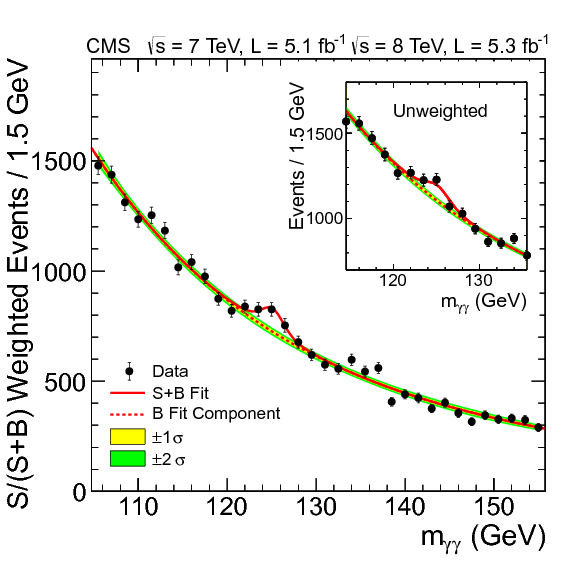
\includegraphics[scale=0.4]{Chapitre5/Images/Hgammagamma.png} 
    \caption{Distribution de la masse invariante diphoton $m_{\gamma\gamma}$ dans les données de la première phase d'exploitation du LHC où chaque évènement est pondéré par son ratio de signal sur signal + bruit de fond S/(S+B) \cite{higgsCMS1}.}
    \label{higgsGG}
\end{figure}

La découverte annoncée en 2012 par les collaborations ATLAS et CMS \cite{CMSdiscovery,ATLASdiscovery},constitue à elle seule une preuve solide de l'existence du boson de Higgs tel que prédit par le mécanisme de Higgs introduit dans le paragraphe \ref{higgsmeca}. La première mesure de sa masse par l'expérience CMS lors de sa découverte est de $m_{H}=125,3\pm0,4(stat.)\pm0,5(syst.)$ GeV dans les canaux $H\rightarrow ZZ\rightarrow 4\ell$ et $H\rightarrow \gamma\gamma$ où l'excès est le plus significatif (Fig. \ref{higgsGG}). Le mode de désintégration en paire de photons permet également de confirmer que la particule observée est un boson de spin différent de 1 et de charge nulle. Les dernières mesures de sa masse par l'expérience CMS offrent désormais une précision à l'ordre du millième avec une valeur $m_{H}=125,38\pm0,14$ GeV dans le canal $H\to\gamma\gamma$ mesurée en 2020 \cite{HiggsMass2020}, puis $m_{H}=125,08\pm0,12$ GeV dans le canal $H\to ZZ\to 4\ell$ mesurée en 2023 \cite{HiggsMass2023}. Parmi les modes de production du boson de Higgs prédits par le modèle standard, 87\% de la section efficace de production au LHC sont attribués à la fusion d'une paire de gluons à travers une boucle quantique de quarks top virtuels (Fig. \ref{Hdecays}.a). Le second mode de production est celui mettant en jeu une fusion de deux bosons vecteurs (Fig. \ref{Hdecays}.b), chacun radié par un des quarks des protons entrés en collision. D'autres modes de production en association avec un boson vecteur (Fig. \ref{Hdecays}.c), ou des quarks de troisième génération (Fig. \ref{Hdecays}.d-f) sont également prédits avec une contribution mineure à la section efficace totale. Le temps de vie du boson de Higgs prédit par le modèle standard est de $\tau_H\approx1,6.10^{-22}$ s, correspondant à une largeur de désintégration $\Gamma_{H}=\hbar/\tau_{H}=4,14\pm0.02$ MeV, définie comme la somme des largeurs de désintégration partielles de tous les modes de désintégration et où $\hbar=h/2\pi$ est la constante de Planck réduite. Dans le modèle standard, ces désintégrations se produisent à travers un couplage à une paire de bosons ou de fermions avec une amplitude proportionnelle à la masse, rendant notamment le couplage aux particules de 3ème génération plus fort. La mesure de la largeur de désintégration est une tâche importante puisqu'une déviation de cette dernière de sa valeur prédite serait une indication directe de nouvelle physique. À ce jour, la mesure réalisée par l'expérience CMS est en accord avec le modèle standard avec une valeur $\Gamma_{H}=3,2^{+2,4}_{-1,7}$ MeV \cite{HiggsWidth2022}. D'autre part, l'expérience CMS observe désormais la désintégration du boson de Higgs en une paire de leptons tau avec $5,9\sigma$, sa désintégration en une paire de quarks $b$ avec $5,6\sigma$, son mode de production associé à une paire de quarks $t$ ($ttH$) avec $5,2\sigma$ et enfin sa désintégration en paire de muons avec $3,0\sigma$ \cite{higgs10years}. Une autre façon de vérifier les prédictions du modèle standard consiste à mesurer une série de paramètres $\kappa$ appelés modificateurs de couplage et associés à chaque vertex faisant intervenir un boson de Higgs (Fig. \ref{Hdecays}). Ces paramètres, dont la valeur prédite dans le modèle standard est de 1 pour tous les couplages, agissent comme des facteurs d'échelle sur les sections efficaces de production et les taux de désintégration du boson de Higgs entre valeurs prédites et valeurs mesurées. La figure \ref{Cmodifiers} présente une mesure des paramètres $\kappa_{V}$ et $\kappa_f$ associés aux couplages aux bosons et fermions massifs respectivement, de la découverte en 2012 à la mesure la plus récente. La mesure des paramètres de couplage individuels pour les bosons $W$ et $Z$, les fermions de 3ème génération et le muon sont également présentés.

\begin{figure}
\centering
    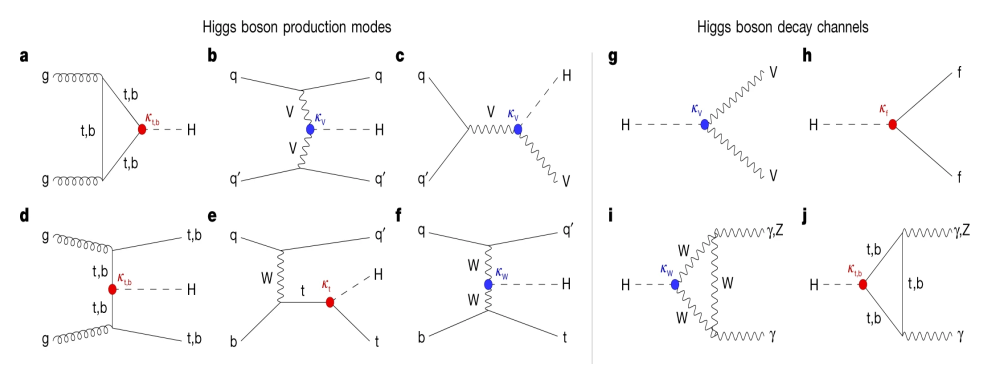
\includegraphics[scale=0.4]{Chapitre5/Images/Hdecays.png} 
    \caption{Diagrammes de Feynmann des (a-f) modes de production du boson de Higgs et des (g-j) modes de désintégration du boson de Higgs \cite{higgs10years}.}
    \label{Hdecays}
\end{figure}

\begin{figure}
\centering
    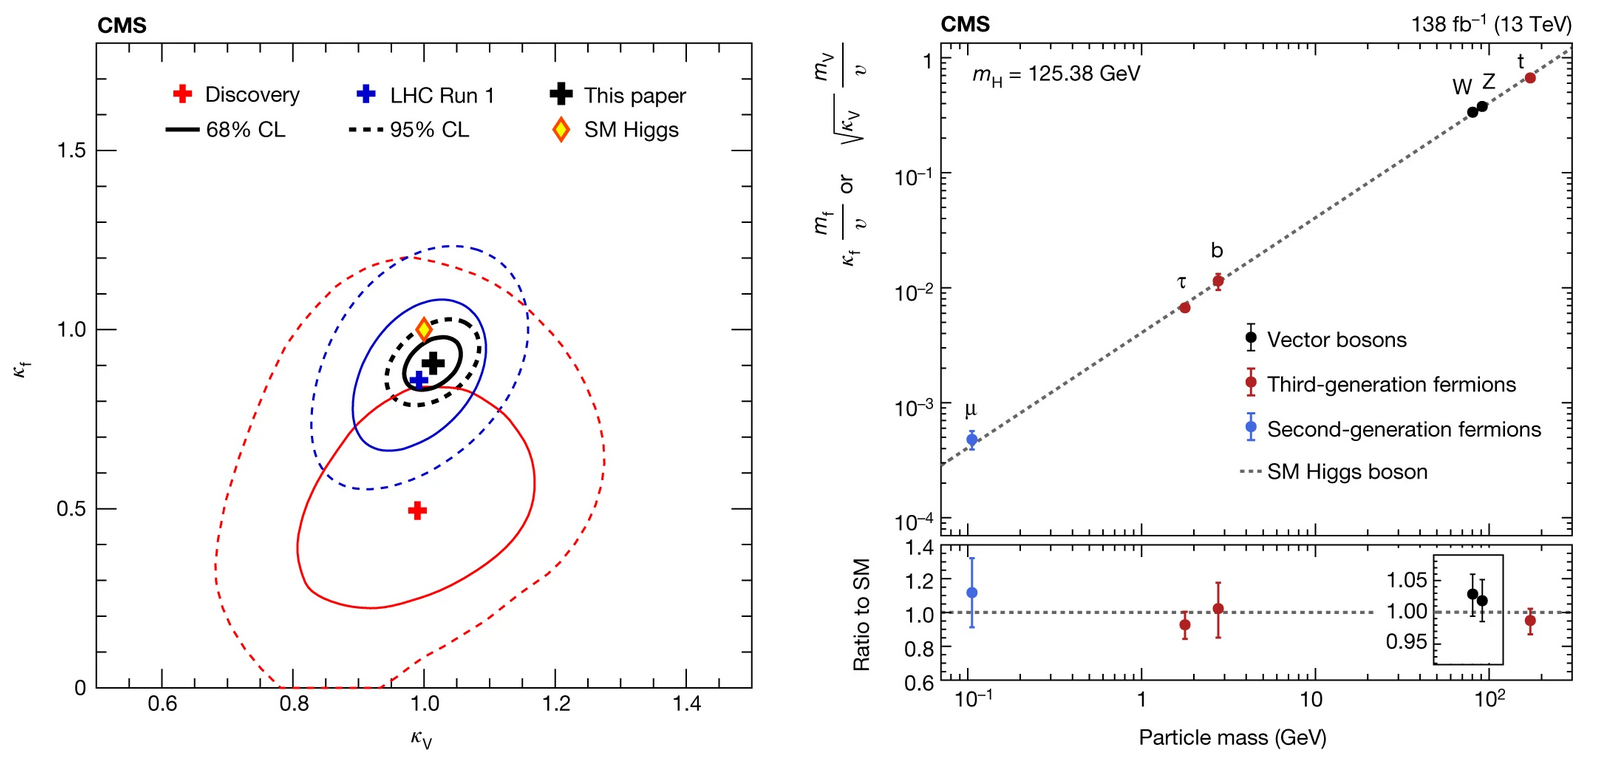
\includegraphics[scale=0.25]{Chapitre5/Images/Cmodifiers.png} 
    \caption{Gauche : contraintes sur la mesure des modificateurs de couplages des fermions ($\kappa_f$) et bosons ($\kappa_V$) depuis sa découverte (rouge), après le Run 1 (bleu) et jusqu'à dix ans après sa découverte (noir). La prédiction du modèle standard est indiquée par le losange jaune. Droite : mesure des modificateurs de couplage bosons vecteurs (noir), des fermions de troisième génération (rouge) et du muon (bleu) en fonction de leur masse \cite{higgs10years}.}
    \label{Cmodifiers}
\end{figure}


\section{Couplage CP impair anomal aux bosons de jauge}
\label{anomalous}

D'après la section \ref{decays}, le boson de Higgs est capable de se coupler aux bosons vecteurs à travers le mode de désintégration $H\rightarrow VV$. Le système final est constitué de deux bosons de nature identique d'état de spin-parité $J^P=1^-$ et possède un moment orbital angulaire total pair tenant compte du spin nul du boson de Higgs initial. Avec ces considérations, le système final est contraint de posséder un état de parité pair, impliquant également une parité paire pour le boson de Higgs dans le cas où la désintégration est invariante sous une transformation CP. Une des analyses de l'expérience CMS menée en 2014 \cite{Z4lCP} porte sur la recherche de violation CP dans le couplage du boson de Higgs au boson $Z$ à travers le mode de désintégration $H\rightarrow ZZ\rightarrow 4l$. La forme la plus générale de l'amplitude de désintégration en paire de bosons vecteurs s'écrit :

\begin{equation}
    \mathcal{A}(H\rightarrow ZZ)=v^{-1}\bigl(a_1m^2_Z\epsilon^*_1\epsilon^*_2+a_2f^{*(1)}_{\mu\nu}f^{*(2),\mu\nu}+a_3f^{*(1)}_{\mu\nu}\tilde{f}^{*(2),\mu\nu}\bigr),
    \label{HZZdecay}
\end{equation}

où $m_Z$ est la masse du boson $Z$, $f^{(i),\mu\nu}=\epsilon_i^{\mu}q_i^{\nu}-\epsilon_i^{\nu}q_i^{\mu}$ est le tenseur champ d'un boson de jauge d'impulsion $q_i$ et de polarisation $\epsilon_i$, $\tilde{f}^(i)_{\mu\nu}\sfrac{1}{2}\epsilon_{\mu\nu\alpha\beta}f^{(i),\mu\nu}$ est le tenseur champ conjugué, $f^*$ son conjugué complexe et $v$ est la v.e.v du champ de Higgs. Les coefficients $a_i$ sont associés à différents couplages. L'amplitude de désintégration est dominée par le couplage associé à $a_1$ pour un couplage CP pair et à $a_3$ pour un couplage CP impair. Afin de mesurer l'accord des données avec une hypothèse de spin-parité quelconque $J^P$ face à celle du modèle standard définie par $J^P=0^+$, on introduit la variable de décision $q$ définie par :

\begin{equation}
    q=-2\ln \frac{\mathcal{L}_{J^P}}{\mathcal{L}_{0^+}},
\end{equation}

où $\mathcal{L}_{J^P}$ est une fonction de vraisemblance associée à l'hypothèse de spin-parité $J^P$ et $\mathcal{L}_{0^+}$ la fonction de vraisemblance associée à l'hypothèse purement scalaire. La figure \ref{statTest} montre la distribution de $q$ attendue pour l'hypothèse purement scalaire en jaune et purement pseudo-scalaire en bleu réalisée à travers de pseudo-expériences simulées. Pour l'hypothèse scalaire (pseudo-scalaire), la fonction de vraisemblance associée est construite en fixant la valeur de tous les coefficients $a_i$ de l'amplitude de désintégration \ref{HZZdecay} à $0$ à l'exception de $a_1$ ($a_3$). La valeur $q_{\text{obs}}$ observée dans les données est marquée par une flèche rouge et favorise de façon claire l'hypothèse purement scalaire en excluant l'hypothèse pseudo-scalaire à $3,8\sigma$.  

\begin{figure}
\centering
    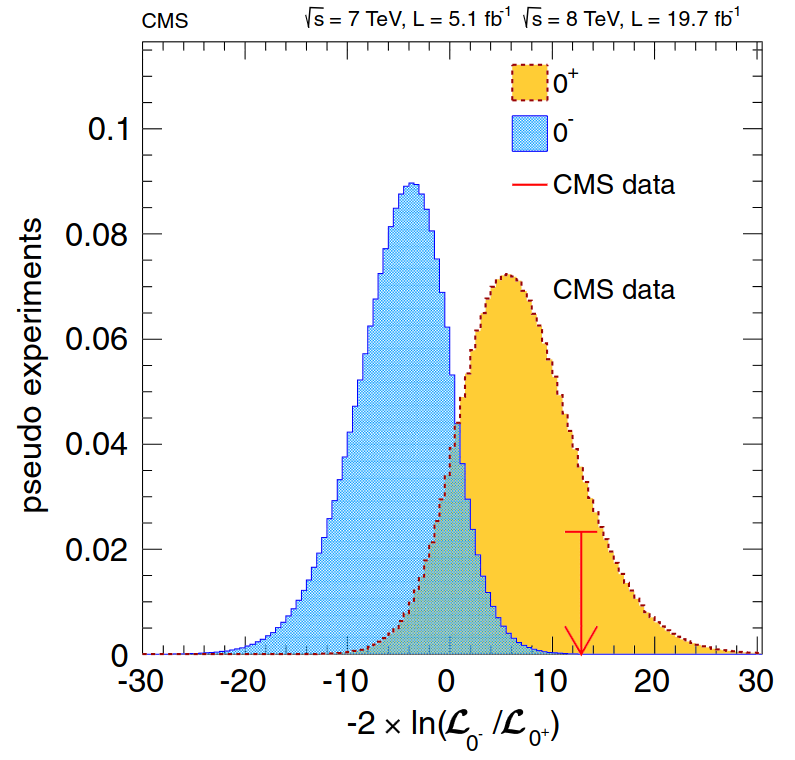
\includegraphics[scale=0.3]{Chapitre5/Images/testStat.png} 
    \caption{Distribution de la variable de décision $q=-2\ln \frac{\mathcal{L}_{0^-}}{\mathcal{L}_{0^+}}$ pour l'hypothèse purement pseudo-scalaire (bleu) face à l'hypothèse purement scalaire (jaune). La flèche rouge indique la valeur observée dans les données du Run 1 \cite{Z4lCP}.}
    \label{statTest}
\end{figure}

\section{Violation de CP dans les couplages de Yukawa}

 Le Lagrangien \ref{yukawacoupling} introduit dans la section \ref{yukawa} reflétant le couplage entre le champ de Higgs et chaque saveur de fermion peut être exprimé de sorte à y faire apparaître une partie scalaire et une partie pseudo-scalaire avec une structure semblable à celle des termes induisant une non conservation de la parité dans les courants chargés de l'interaction faible :

    \begin{equation}
        \mathcal{L}_Y = -\frac{m_f}{\nu}\bigl(\kappa_f\overline{\psi}\psi+\tilde{\kappa}_f\overline{\psi}i\gamma^5\psi\bigr)h,
    \end{equation}

    où $\kappa_f$ représente un paramètre propre au couplage scalaire, et $\tilde{\kappa}_f$ un paramètre propre au couplage pseudo-scalaire. Ces constantes permettent alors de définir une fraction pseudo-scalaire $f^{Hff}_{CP}$ du couplage, pouvant elle-même être librement exprimée en fonction d'un angle de mélange $\alpha^{Hff}$ :

    \begin{equation}
        f^{Hff}_{CP}=\frac{|\tilde{\kappa}_f|^2}{|\kappa_f|^2+|\tilde{\kappa}_f|^2}=\sin^2(\alpha^{Hff}).
    \end{equation}

    Dans le cadre du modèle standard où le boson de Higgs est une particule purement scalaire, les paramètres $\kappa_f$ et $\tilde{\kappa}_f$ sont définis tels que 

    \begin{equation*}
    \boxed{
        \kappa_f=1 \quad \mbox{et} \quad \tilde{\kappa}_f=0.
    }
    \end{equation*}

    De cette façon, l'angle de mélange possède une valeur nulle et seule le terme scalaire participe dans le couplage aux fermions. À l'inverse, un angle de mélange de $90^\circ$ reflète un couplage purement pseudo-scalaire tandis que toute valeur arbitraire représente une mixture des deux couplages avec un maximum de mélange pour un angle de $45^\circ$, lorsque $\kappa_f=\tilde{\kappa}_f=0.5$. \\

    \subsection{Mode de production $t\overline{t}H$}

    En 2020, la collaboration CMS a publié un article dans lequel la structure CP du couplage de Yukawa du quark top est étudiée \cite{ttH}. L'analyse se concentre sur le mode de production associé à une paire $t\overline{t}$ (Fig. \ref{Hdecays}.d) avec un état final $H\rightarrow\gamma\gamma$. La présence d'une paire de quarks top donne lieu à deux canaux distincts avec des critères de sélection spécifiques :

    \begin{itemize}
        \smallskip
        \item[$\bullet$] Canal leptonique, avec présence d'au moins un lepton ($e/\mu$) isolé et présence d'au moins un jet de hadrons.
        \smallskip
        \item[$\bullet$] Canal hadronique, avec présence d'au moins trois jets de hadrons dont au moins un est issu d'un quark $b$ et absence de lepton ($e/\mu$) isolé.
        \smallskip
    \end{itemize}

        \begin{figure}
    \centering
    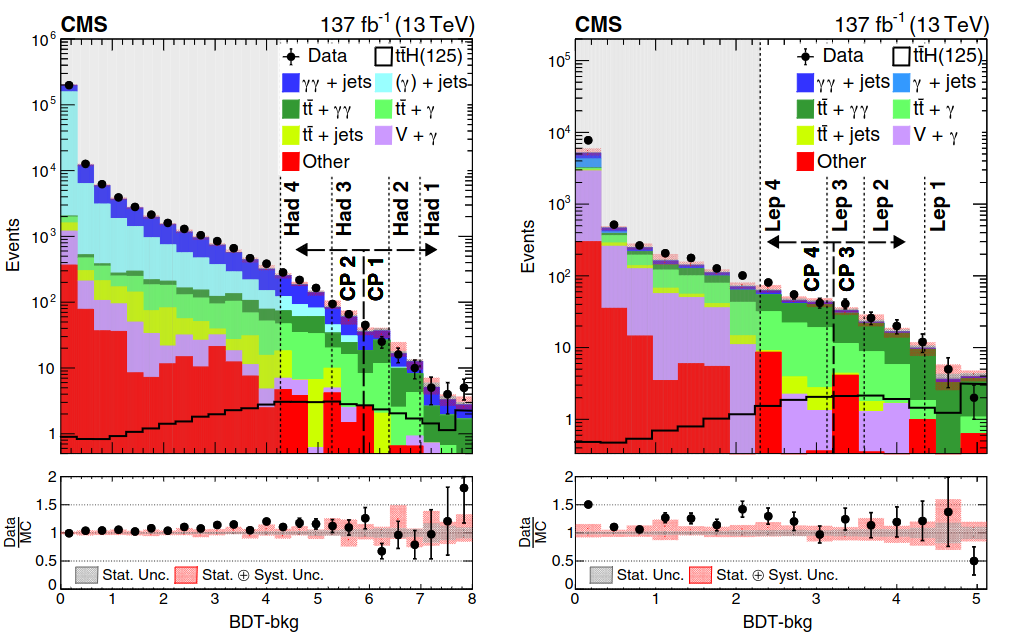
\includegraphics[scale=0.35]{Chapitre5/Images/BDTbkg.png} 
    \caption{Distribution du score de sortie de BDT-bkg dans le canal hadronique (gauche) et leptonique (droite). Seuls les évènements à droite des zones grises sont conservés. Les catégories utilisées pour la mesure de $\mu_{ttH}$ ($f_{CP}^{Htt}$) sont séparées par la ligne discontinue fine (épaisse) \cite{ttH}.}
    \label{BDTbkg}
\end{figure}

    Les bruits de fonds principaux pour ces évènements sont notamment la production directe de photons associée à des jets ($\gamma+jets$, $\gamma\gamma+jets$), la production directe d'une paire $t\overline{t}$ associée à des photons ou des jets ($t\overline{t}+\gamma$, $t\overline{t}+\gamma\gamma$, $t\overline{t}+jets$) et la production d'un boson vecteur associée à un photon ($W+\gamma$, $Z+\gamma$), ainsi que les autres modes de production du boson de Higgs. Un arbre de décision boosté (BDT) est employé dans chaque canal (leptonique, hadronique) afin d'effectuer une classification des évènements entre signal et bruit de fond. Ces deniers utilisent notamment en entrée les propriétés cinématiques des leptons, photons, jets et du système di-photon de chaques évènements, et à l'exception de la masse invariante $m_{\gamma\gamma}$ qui constitue l'observable de cette analyse. D'autres variables sont également utilisées comme la multiplicité des jets et des leptons, le score d'identification des jets de quarks $b$ et l'impulsion transverse manquante. La figure \ref{BDTbkg} présente la distribution du score de sortie du BDT (BDT-bkg) dans chaque canal ainsi que l'accord entre les données du Run 2 et l'estimation du bruit de fond réalisée par simulation Monte Carlo. Les évènements non rejetés ayant passé un certain seuil de score sont par la suite répartis en huit catégories destinés à la mesure de l'intensité du signal $\mu_{ttH}$ à travers un ajustement simultané de la distribution de la masse invariante $m_{\gamma\gamma}$. Quatre catégories (CP1, CP2, CP3, CP4) sont également définies afin d'optimiser la sensibilité à la structure CP du couplage dans chacune d'elle. Chacune de ces catégories est ensuite séparée en trois autres selon la valeur de l'observable $\mathcal{D}_{0^-}$ fournie par un second BDT destiné à séparer les contributions CP paires et impaires. Un second ajustement simultané de la distribution de la masse invariante $m_{\gamma\gamma}$ utilisant les douze catégories est ainsi réalisé permettant d'extraire une valeur $f_{CP}^{Htt}=0,00\pm0,33$ à un niveau de confiance de $68$\% et d'exclure l'hypothèse $f_{CP}^{Htt}=1$ à $3,2\sigma$.


    \subsection{Désintégration $H\rightarrow\tau\tau$}
    \label{Htautau}
    
    Par conservation du moment angulaire, le spin nul du boson de Higgs impose une valeur nulle à la somme des composantes longitudinales $s_{z}^{\pm}$ du spin des deux fermions dans la désintégration $H^0\rightarrow\tau\tau$. Cette contrainte laisse la corrélation entre les deux composantes transverses $s_{\perp}^{\pm}=\sqrt{s_{x}^{\pm2}+s_{y}^{\pm2}}$ du spin pour seul effet sensible à l'état CP pair ou impair. Selon le même principe illustré dans le paragraphe \ref{verslarelat}, l'information sur les composantes $s_x$ et $s_y$ du spin dans le plan transverse est perdue. Toute fois dans le cas d'un couplage scalaire, l'alignement des composantes transverses du spin sera favorisé et inversement leur anti-alignement sera favorisé dansle cas d'un couplage pseudo-scalaire. L'expression du taux de désintégration $H^0\rightarrow\tau\tau$ s'exprime alors selon :

    \begin{equation}
    \Gamma(H^0\rightarrow\tau\tau)\propto1-s_{z}^-s_{z}^++s_{\perp}^-R(\alpha^{H\tau\tau})s_{\perp}^+,
    \end{equation}

    où $s$ est le spin des leptons tau, et $R$ est une matrice dépendante de l'angle de mélange $\alpha^{H\tau\tau}$ agissant sur la corrélation des composantes transverses du spin. Plusieurs méthodes initialement prévues pour des études sur collisionneur électron-positron ont été développées au début des années 2000 \cite{Desch_2003,Desch_2004}. Bien que ce type de collisionneur présente l'avantage d'une reconstruction simplifiée du référentiel au repos du boson de Higgs, la section \ref{CPmethods} présente les méthodes déployées au LHC. Ces méthodes ont notamment été utilisées dans la première analyse de la structure du couplage de Yukawa du lepton tau avec les données du Run 2 réalisée par CMS \cite{Htautau}. Les résultats de cette analyse sont présentés dans la figure \ref{Htautauresults} et montrent la mesure de l'intensité du signal $$\mu=\mu_{ggH}=\mu_{qqH}=\frac{\sigma_{qqH/ggH}\times\mathcal{B}_{\tau\tau}}{(\sigma_{qqH/ggH}\times\mathcal{B}_{\tau\tau})_{SM}},$$ de l'angle de mélange $\alpha^{H\tau\tau}$ et des constantes de couplages $\kappa_{\tau}/\tilde{\kappa}_{\tau}$. L'hypothèse pseudo-scalaire est exclue à $3,0\sigma$ dans les données, et l'angle de mélange est mesuré avec une valeur de $\alpha^{H\tau\tau}=-1\pm19^\circ$ à un niveau de confiance de $68,3$\%. \\

\begin{figure}
    \begin{subfigure}[b]{0.5\linewidth}
        \centering
        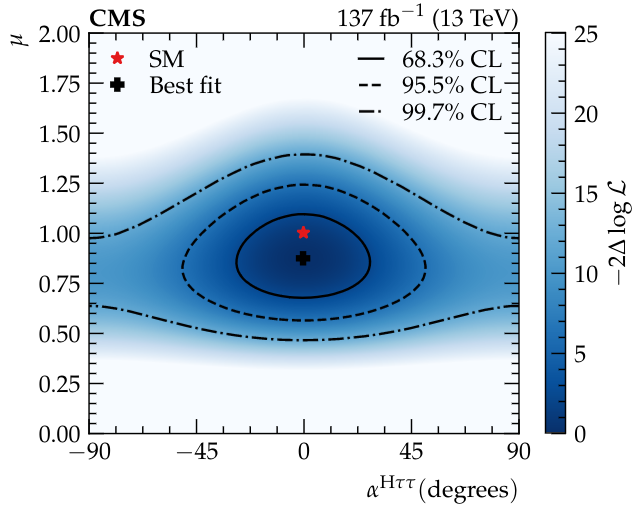
\includegraphics[width=\linewidth]{Chapitre5/Images/AlphaHtt.png}
    \end{subfigure}
    \begin{subfigure}[b]{0.5\linewidth}
        \centering
        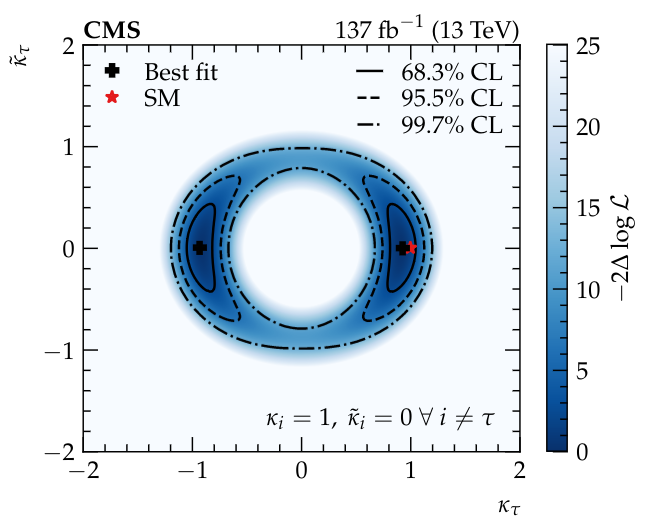
\includegraphics[width=\linewidth]{Chapitre5/Images/kappaHtt.png}
    \end{subfigure}
    \caption{Gauche : mesure des paramètres $\mu$ vs $\alpha^{H\tau\tau}$. Droite : mesure des paramètres $\tilde{\kappa}_{\tau}$ vs $\kappa_{\tau}$ \cite{Htautau}.}
    \label{Htautauresults}
\end{figure}

La mesure du paramètre $\tilde{\kappa}_{\tau}$ et ainsi la contribution pseudo-scalaire au couplage de Yukawa du lepton tau peut également être contrainte par la mesure du moment dipolaire électrique (EDM) du neutron et de l'électron \cite{Brod2013}. Le couplage pseudo-scalaire du lepton tau au boson de Higgs entraîne notamment l'apparition d'un EDM $d_\mathrm{e}$ pour l'électron à travers le diagramme présenté dans la figure \ref{barrzee} et dont le Lagrangien effectif s'écrit :

\begin{equation}
    \mathcal{L}_{\text{eff}}=-d_\mathrm{e}\frac{i}{2}\overline{\mathrm{e}}\sigma^{\mu\nu}\gamma_5\mathrm{e}F_{\mu\nu}.
\end{equation}

Ce Lagrangien représente la limite relativiste de l'Hamiltonien décrivant l'interaction entre une particule de spin $S=\sfrac{1}{2}$ tel que l'électron et un champ électrique $\vb{E}$ tel que décrit dans la référence \cite{Pospelov_2005} : $$H=-d_\mathrm{e}\vb{E}\cdot\frac{\vb{S}}{S}.$$ Avec une valeur non nulle de $d_\mathrm{e}$, ce terme est responsable d'une violation de la symétrie du temps $T$, et par conservation de la symétrie $CPT$, implique également une violation de la symétrie $CP$. La relation entre $d_\mathrm{e}$ et $d_n$, les EDM de l'électron et du neutron respectivement, et le couplage $\tilde{\kappa}_{\tau}$ s'exprime pour chacune :

\begin{align}
    d_\mathrm{e}&=3,7\cdot10^{-29}[e.\text{cm}]\times\tilde{\kappa}_{\tau},
    \label{constraint1} \\
    d_n&=(1,0\pm0,5)\cdot22,3\cdot10^{-29}[e.\text{cm}]\times\tilde{\kappa}_{\tau},
    \label{constraint2}
\end{align}

où $e$ est la charge électrique élémentaire. Les dernières mesures imposent une valeur limite $|d_\mathrm{e}|<1,1\cdot10^{-29}$ $e.\text{cm}$ pour l'électron \cite{eEDM} et $|d_n|<1,8\cdot10^{-26}$ $e.\text{cm}$ pour le neutron \cite{nEDM}. Grâce aux équations \ref{constraint1} et \ref{constraint2}, la plus forte contrainte sur la valeur découle de la mesure de l'EDM de l'électron en imposant $\tilde{\kappa}_{\tau}<0,3$.

\begin{figure}
\centering
    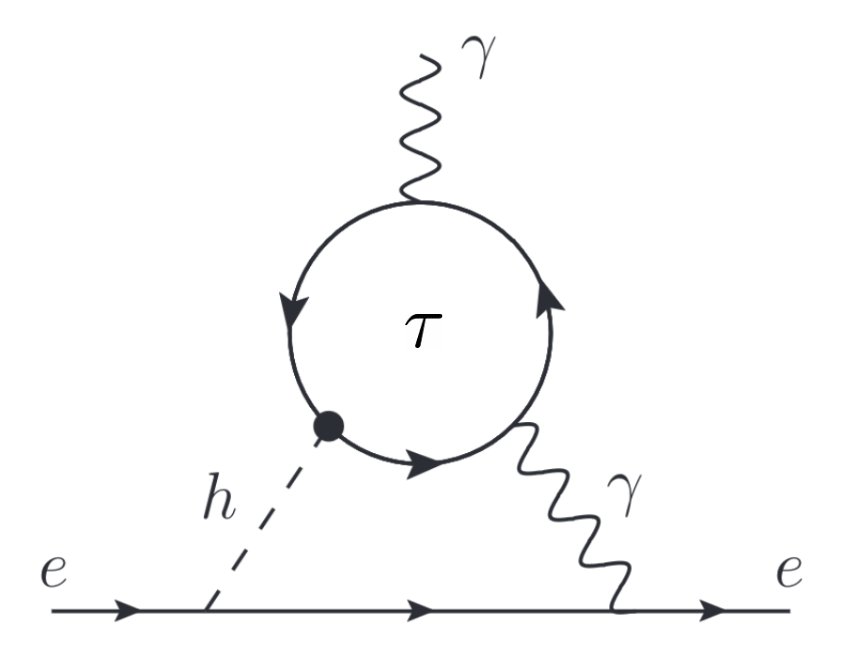
\includegraphics[scale=0.25]{Chapitre5/Images/barrzee.png} 
    \caption{Diagramme de Barr-Zee contribuant au moment dipolaire de l'électron \cite{barrzee}.}
    \label{barrzee}
\end{figure}
